\documentclass[informe,english]{plantilla}
\usepackage[background]{lst-shell}
\usepackage[background]{lst-c}
\usepackage[background]{lst-python}

\usepackage{graphicx}
\usepackage{amsmath}
\usepackage{amsfonts}
\usepackage{amssymb}
\usepackage{enumitem}
\usepackage{float}
\usepackage{textcomp}

\title{Weather station system}
\assignatura{Internet of Things Connectivity}
\subtitle{Activity 2: LoRa-based communication with MQTT integration ---
  \textsf{Internet of Things Connectivity}}
\numpract{2}
\autor{Aarón Alcalá \and Marcos García \and Jaume Pulido \and Mikael Rodríguez}
\date{\today}

% Footer strings in English (the class writes them in\ Catalan by default)
\makeatletter
\ifoot[Report~\practno.~\@assignatura]{%
  \def\and{, }\@author. Report~\practno.~\@assignatura}
\ofoot[\pagemark]{\pagemark}
\makeatother

% custom commands
\newcommand{\tcmp}[1]{\textlangle #1\textrangle}

\newcommand{\img}[8]{%
\begin{figure}[h]
\begin{center}
\includegraphics[trim=#4cm #5cm #6cm #7cm, clip,width=#3\textwidth]{#1} \\ % trim=left bottom right top
\caption{#2}
\label{fig:#8}
\end{center}
\end{figure}
}

\lstdefinelanguage{ini}{
  sensitive=false,
  morecomment=[l]{;},
  morestring=[b]"
}

\lstset{
  style=lst-common,
  backgroundcolor=\color{upcblue!8!white},
  basicstyle=\ttfamily\footnotesize,
  breaklines=true,
  postbreak=\mbox{\textcolor{upcred}{$\hookrightarrow$}\space},
  captionpos=b,
  keywordstyle=\color{upcblue}\bfseries,
  aboveskip=5pt,
  belowskip=5pt,
}

% ---- Needed by the TX / Experiments part (Jaume) ----
\usepackage[T1]{fontenc}   % so { } show correctly in \texttt
\usepackage{booktabs}
\usepackage{pgfplots}
\pgfplotsset{compat=1.17}

% Red marker for things still to fill in after the experiments
\providecommand{\todo}[1]{\textcolor{red}{\textbf{[TODO: #1]}}}

\lstdefinestyle{arduino}{
    language=C++,
    basicstyle=\ttfamily\footnotesize,
    keywordstyle=\color{blue!70!black}\bfseries,
    commentstyle=\color{green!45!black}\itshape,
    stringstyle=\color{orange!80!black},
    numbers=left, numberstyle=\tiny\color{gray},
    frame=single, breaklines=true, showstringspaces=false,
    tabsize=4, captionpos=b
}

\begin{document}
\newpage

% =====================================================================
\section{Introduction}
\label{sec:intro}
% =====================================================================
This report documents Activity 2 of the Weather station system, which extends the MQTT chain of Activity 1 by introducing a LoRa link between two ESP32 boards: a transmitter (TX) node that reads the DHT11 sensor and sends the data over LoRa, and a receiver (RX) node that forwards what it receives to the Mosquitto broker over MQTT, so that the dashboard remains unchanged.

For this activity, two groups joined forces: Aarón Alcalá and Marcos García on one side, and Jaume Pulido and Mikael Rodríguez on the other. The work was split so that each group programmed one of the two nodes. Jaume and Mikael's group developed the TX node, including the handling of the DHT11 sensor, and Aarón and Marcos's group developed the RX node, where the WiFi connection, the MQTT publication to the Mosquitto broker and the web frontend keep the same idea and structure as in Activity 1.
 
% =====================================================================

\section{LoRa Configuration}

The LoRa communication system enables two ESP32-based boards to exchange sensor information wirelessly. The objective is to provide a long-range communication link suitable for IoT applications while keeping the implementation modular and easy to maintain.

The configuration and communication logic are separated into different files. The \texttt{LoRaConfig.h} file defines the radio configuration structure, while \texttt{config.h} contains the default radio parameters and hardware pin assignments. The \texttt{LoRa\_IOT.h} and \texttt{LoRa\_IOT.cpp} files define the communication interface and its implementation. This separation allows the radio parameters to be modified without changing the application logic.

\subsection{Radio Parameters}

The radio configuration is centralised in \texttt{config.h} and passed to the initialisation function through the \texttt{LoRaConfig} structure. The main parameters and their design rationale are described below.

\begin{itemize}
    \item \textbf{Frequency (868 MHz):}
    Selected for operation in the European 868 MHz band, subject to applicable regulations. Both boards must use the same frequency     to communicate.

    \item \textbf{Bandwidth (250 kHz):}
    Provides a relatively high data rate compared with narrower bandwidths, making it suitable for transmitting small sensor
    messages periodically.

    \item \textbf{Spreading factor (SF7):}
    Selected to favour a higher data rate and shorter transmission times. This is suitable for small sensor messages, provided that the required communication range and signal quality are maintained.

    \item \textbf{Coding rate (4/5):}
    Adds forward error correction to improve resilience against transmission errors while limiting additional transmission overhead.

    \item \textbf{Sync word (0x12):}
    Helps distinguish our LoRa network from networks using different sync words. Both boards must use the same value.

    \item \textbf{Preamble length (8 symbols):}
    Supports packet detection and synchronisation while limiting transmission overhead.

    \item \textbf{CRC enabled:}
    Allows the receiver to detect corrupted packets and identify yransmission errors.
\end{itemize}

The transmit power is also configurable. Its final value must bec ompatible with the radio module and comply with the applicable regional regulations.

\subsection{Network Compatibility and Interference}

Reliable communication requires both ESP32 boards to use compatible radio parameters, including frequency, bandwidth, spreading factor, coding rate, and sync word. Centralising these values ensures consistency and simplifies configuration changes.

The selected sync word helps distinguish our network from other LoRa networks using different settings. However, LoRa operates over a shared radio channel, meaning that other devices transmitting on the same frequency may still cause interference or packet collisions. Therefore, this configuration reduces the likelihood of accepting packets from unrelated networks but cannot guarantee exclusive communication between our two boards.

Furthermore, the sync word does not provide encryption or sender authentication. Additional security mechanisms would be required if confidentiality or protection against unauthorised transmissions were necessary.

\subsection{Software Design}

The communication software follows a modular design, separating radio configuration from the application that processes sensor data. The public interface provides functions for initialisation, transmission, and reception, while the implementation manages the radio hardware through the Arduino LoRa library.

This approach simplifies integration with the rest of the IoT application and allows the communication layer to be maintained independently. A GPIO interrupt is also configured to signal radio events, keeping the interrupt handler lightweight. In the current implementation, packet reception is handled through polling, while the interrupt flag is not yet integrated into the reception logic.

Overall, the selected configuration establishes a common radio profile for both boards, while the modular software structure
facilitates maintenance and future adaptation. The final parameters should be validated under the expected operating distances and environmental conditions.

\section{LoRa library}
\label{sec:lora-lib}

% ASSIGNED: MIKA
% Files: LoRaIOT.hh / LoRaIOT.cpp / LoRaConfig.h / config.h
% =====================================================================
\tcmp{Introducción breve: por qué se encapsula LoRa en una librería propia (\texttt{LoRaIOT}) y qué problema resuelve.}

\subsection{LoRaIOT class (\texttt{LoRaIOT.hh} / \texttt{LoRaIOT.cpp})}
\tcmp{Interfaz pública, funciones principales (inicialización, envío, recepción), librería base usada.}

\subsection{LoRa parameters (\texttt{LoRaConfig.h})}
\tcmp{Parámetros configurables: frecuencia, spreading factor, bandwidth, coding rate, potencia de transmisión, sync word\ldots}

\subsection{General configuration (\texttt{config.h})}
\tcmp{Pines del módulo LoRa, parámetros comunes entre TX y RX, intervalo de envío.}

% =====================================================================
\section{TX node (\texttt{src/tx/main.cpp})}
\label{sec:tx}
% ASSIGNED: JAUME
% =====================================================================

The transmitter is the node placed at the weather station. Its only task is to read the DHT11 sensor periodically and send each reading over LoRa to the receiver, which acts as a gateway towards the MQTT broker. Because it does not need any Internet connectivity, the transmitter does not use WiFi or MQTT at all, which keeps the firmware small and reduces its power consumption.

The program is built with PlatformIO in its own environment (\texttt{env:tx}), which compiles only the \texttt{src/tx/} folder through
\texttt{build\_src\_filter}. The radio code is shared with the receiver and lives in the \texttt{lib/lora} library (\texttt{LoRa\_IOT.h/.cpp}), so the main file only contains the application logic.

\subsection{Configuration}

All the parameters are defined in \texttt{include/config.h} and loaded into a \texttt{LoRaConfig} structure (\texttt{lib/lora/LoRaConfig.h}), whose default values come from these macros. Both nodes use the same structure, which guarantees that they share the same radio settings. Table~\ref{tab:lora-config} summarises the values used.

\begin{table}[h]
    \centering
    \begin{tabular}{@{}ll@{}}
        \toprule
        \textbf{Parameter}        & \textbf{Value} \\
        \midrule
        Board / radio             & Heltec WiFi LoRa 32 V2 / SX1276 \\
        Frequency                 & 868~MHz (EU868) \\
        Bandwidth                 & 250~kHz \\
        Spreading factor          & 7 \\
        Coding rate               & 4/5 \\
        Preamble length           & 8 symbols \\
        Sync word                 & \texttt{0x12} \\
        TX power (default)        & 20~dBm \\
        CRC                       & Enabled \\
        Sensor                    & DHT11 on GPIO~13 \\
        Send interval             & 5~s (\texttt{LORA\_SEND\_INTERVAL\_MS}) \\
        \bottomrule
    \end{tabular}
    \caption{LoRa and application parameters used by the transmitter.}
    \label{tab:lora-config}
\end{table}

\subsection{Initialisation}

The \texttt{setup()} function opens the serial port for debugging, starts the
DHT11 driver and initialises the radio with \texttt{LoRaIOT\_setup()}:

\begin{lstlisting}[style=arduino, caption={Initialisation of the transmitter.}]
DHT dht(DHT_PIN, DHT_TYPE);
LoRaConfig loraConfig;                  // default values from config.h
int counter = 0;                        // packet id

void setup(){
    Serial.begin(115200);
    dht.begin();

    if (!LoRaIOT_setup(loraConfig))
        while (1);                      // stop if the radio does not answer
}
\end{lstlisting}

\texttt{LoRaIOT\_setup()} starts the SPI bus on the pins of the on-board SX1276, sets the chip-select, reset and DIO0 pins, calls
\texttt{LoRa.begin()} with the carrier frequency and then applies the spreading factor, bandwidth, coding rate, preamble length, sync word and transmission power, and enables the CRC. If the radio does not respond, the function returns \texttt{false} and the program stops, since the node is useless without the radio.

\subsection{Main loop}

Every iteration of \texttt{loop()} performs three steps: it reads the sensor, builds the message and sends it.

\begin{lstlisting}[style=arduino, caption={Main loop of the transmitter.}]
void loop(){
    float temperature = dht.readTemperature();
    float humidity    = dht.readHumidity();

    if (isnan(temperature) || isnan(humidity)) {
        Serial.println("Error leyendo el DHT11");
        delay(2000);
        return;                         // retry without sending anything
    }

    String message = "{\"id\":" + String(counter) + ",\"temperature\":" + String(temperature, 1) + ",\"humidity\":" + String(humidity, 1) + "}";

    if (!LoRaIOT_send(message))
        Serial.println("Error enviando el paquete");

    counter++;
    delay(LORA_SEND_INTERVAL_MS);
}
\end{lstlisting}

\paragraph{Sensor reading.} The DHT11 returns \texttt{NaN} when a reading fails (for example, if it is read too often or a wire is loose). In that case the iteration is discarded and repeated after 2~s, so invalid values are never transmitted.

\paragraph{Message format.} Each reading is encoded as a small JSON object:
\begin{center}
    \texttt{\{"id":12,"temperature":23.4,"humidity":55.0\}}
\end{center}
Values are rounded to one decimal, which matches the resolution of the DHT11. JSON was chosen because the receiver can parse it directly with ArduinoJson and the format is easy to read in the serial monitor. The field \texttt{id} is a counter that increases with every packet; the receiver can use it to detect lost packets by looking for gaps in the sequence. The message is about 43--45~bytes long, far below the 255-byte limit of a LoRa packet. 

\paragraph{Transmission.} \texttt{LoRaIOT\_send()} wraps the three calls of the Arduino LoRa library: \texttt{beginPacket()}, \texttt{print()} and \texttt{endPacket()}. The last one is blocking: it returns when the radio signals the end of the transmission (\emph{TxDone}), so when \texttt{LoRaIOT\_send()} returns the packet has already been sent.

\paragraph{Send period.} After each packet the node waits \texttt{LORA\_SEND\_INTERVAL\_MS} (5~s). This respects the DHT11 minimum
sampling period (1~s) and keeps the channel occupancy low: with a time on air of around 44~ms (see Section~\ref{sec:exp-toa}), the duty cycle is below 1\%, which is the limit of the EU868 sub-band used.

% =====================================================================
\section{RX node}
\label{sec:rx}

% ASSIGNED: MARCOS

% (más adelante se simplificará hacia las partes más básicas)

% =====================================================================

The RX node is the bridge between the LoRa link and the MQTT chain built in Activity 1. Its task is to wait for the packets sent by the TX node, extract the temperature and humidity from them and republish them to the Mosquitto broker, so that the dashboard keeps working exactly as before. The WiFi connection, the MQTT publication and the web frontend follow the same idea and structure as in Activity 1, so the only new element on this node is the LoRa reception.

\subsection{Main program (\texttt{main.cpp})}

The program is built with PlatformIO in its own environment (\texttt{env\:rx}), which compiles only the \texttt{src/rx/} folder through \texttt{build\_src\_filter}. 

The \texttt{main.cpp} of the RX node reuses the \texttt{WiFiManager} and \texttt{MqttPublisher} classes of Activity 1 and adds the LoRa functions provided by the library described in Section~\ref{sec:lora-lib}. Besides the WiFi and MQTT objects, the program only needs one extra global variable, \texttt{rxFlag}, a \texttt{volatile bool} that signals that a LoRa packet has arrived.

\paragraph{Initialization.} In \texttt{setup()}, the WiFi manager is started as in Activity 1, and the radio is configured through \texttt{LoRaIOT\\\_setup(LoRaConfig())}. This is the same call used by the TX node, so both boards share exactly the same radio configuration (frequency, spreading factor, bandwidth, coding rate, preamble length and sync word); otherwise the receiver would not be able to decode the packets. If the radio fails to start, the program stops, since the node would be useless without it. Finally, \texttt{LoRa.receive()} is called to put the radio in continuous receive mode. This call is essential: after \texttt{LoRa.begin()} the module is not listening by default, so without it no packet would ever be detected and the interrupt described below would never fire.

\paragraph{Interrupt-driven reception.} Instead of repeatedly asking the radio whether a packet has arrived, the RX node relies on a hardware interrupt. An interrupt makes the microcontroller run a function only when a given event happens, which here is the arrival of a packet. During \texttt{LoRaIOT\\\_setup()}, \texttt{attachInterrupt()} associates the DIO0 pin of the LoRa module with the function \texttt{onLoRaRxIRQ()}, which is executed on every rising edge of that pin, i.e.\ when the module signals that a complete packet has been received:

\begin{lstlisting}[style=arduino]
extern volatile bool rxFlag;

void IRAM_ATTR onLoRaRxIRQ()
{
    // The interrupt only signals that a packet has arrived
    rxFlag = true;
}
\end{lstlisting}

The interrupt routine does nothing but raise the flag, since this kind of routine must be as short as possible. The variable is declared \texttt{volatile} in \texttt{main.cpp} because it is modified from the interrupt and read from \texttt{loop()}, so the compiler must not assume that its value stays unchanged between reads. The library file accesses it through \texttt{extern}, and the \texttt{IRAM\\\_ATTR} attribute keeps the routine in the ESP32 internal RAM so it can run quickly. The heavy work (reading the packet, parsing it and publishing it) is done later in the main loop, outside the interrupt.

\paragraph{Main loop.} On every iteration, \texttt{loop()} follows these steps:

\begin{enumerate}[noitemsep]

    \item The WiFi manager is updated, and the iteration is skipped if there is no connection yet.

    \item If the MQTT connection has not been established, it is attempted again, and \texttt{mqttPublisher.loop()} is called to keep it alive. These steps work exactly as in Activity 1.

    \item If \texttt{rxFlag} is set, it is cleared first and then the packet is read with \texttt{LoRaIOT\\\_receive()}.

    \item If a packet was read correctly and the MQTT connection is available, the message is handed to \texttt{publishReading()}.

\end{enumerate}

In contrast with Activity 1, the publication is no longer periodic: nothing is sent to the broker until a LoRa message arrives, so the publishing rate is set by the TX node.

\paragraph{Packet reception.} The \texttt{LoRaIOT\_receive()} function checks for an incoming packet using \texttt{LoRa.parsePacket()}. If no packet is available, it returns \texttt{false}. Otherwise, it reads the packet byte by byte using \texttt{LoRa.available()} and \texttt{LoRa.read()}, storing the received data in the \texttt{message} string. It then prints the message and its RSSI value, which indicates the received signal strength. Finally, \texttt{LoRa.receive()} puts the radio back into reception mode, and the function returns \texttt{true} to indicate that a packet has been received.


\paragraph{From the LoRa message to MQTT.} The message received over LoRa is a JSON string. \texttt{publishReading()} deserializes it with \textit{*ArduinoJson*}, discarding the packet and reporting the error if the parsing fails. Then it extracts only the temperature and the humidity, ignoring the rest of the fields of the received JSON, such as the packet counter \texttt{id}, since that information is not going to be sent over MQTT. Finally, it builds a new JSON with the \texttt{temp} and \texttt{hum} fields through the \texttt{MqttPublisher} and publishes it to the broker:

\begin{lstlisting}[style=arduino]
StaticJsonDocument<200> doc;
DeserializationError error = deserializeJson(doc, message);

if (error) return false;
float temperature = doc["temperature"];
float humidity = doc["humidity"];

publisher.addField("temp", temperature);
publisher.addField("hum", humidity);
publisher.publish(topic, retained);
\end{lstlisting}

Rebuilding the JSON with the same fields as in Activity 1 is what allows the rest of the chain to remain unchanged: the broker and the dashboard receive the same message on \texttt{sensor/1} as if the sensor were connected directly to the node.

\subsection{MQTT}

The MQTT part of the RX node is the same as in Activity 1. The \texttt{WiFiManager} state machine handles the connection to the WiFi network without blocking, and the \texttt{MqttPublisher} class connects to the Mosquitto broker, reconnects automatically if the connection is lost, and serializes and publishes the JSON message. The only difference is that the readings now come from the LoRa packets instead of a local sensor.

\subsection{Frontend}

The frontend does not change either. \texttt{dashboard.py} keeps subscribing to \texttt{sensor/+}, storing the readings in bounded queues and drawing the live charts with Dash and Plotly, as described in Activity 1. Since the RX node publishes the same JSON format and topic, the dashboard cannot tell whether the data comes from a sensor wired to the node or from a remote one over LoRa.

% =======

% =====================================================================
\section{Experiments}
\label{sec:experiments}
% ASSIGNED: JAUME / AARON
% (preparar el documento de experimentos + redactar esta parte)
% =====================================================================
\subsection{Transmission power vs.\ energy consumption and signal strength}
\label{sec:exp-txpower}

The aim of this experiment is to evaluate how the transmission power affects the signal strength at the receiver and the energy that the transmitter needs to send each packet. In a battery-powered sensor node there is a trade-off between both: a higher power gives a stronger and more robust link, but drains the battery faster.

\subsubsection{Test procedure}

The experiment is automated with a PlatformIO test, \texttt{test/test\_tx\_power/test\_tx\_power.cpp}, written with the Unity framework. It runs on the transmitter board and is launched with its own environment, \texttt{env:tx\_power}, which extends \texttt{env:tx} and only runs this test:
\begin{center}
    \texttt{pio test -e tx\_power}
\end{center}

The test performs the following steps:
\begin{enumerate}
    \item It initialises the radio with \texttt{LoRaIOT\_setup()} and the same configuration as the normal firmware
          (Table~\ref{tab:lora-config}). If this fails, the test fails.
    \item For each power level in $\{2, 5, 8, 11, 14, 17, 20\}$~dBm, it sets the power with \texttt{LoRa.setTxPower()} and sends 10 packets, 500~ms apart. Each packet carries the power used and a sequence number, so the receiver can tell which level it belongs to:
          \begin{center}
              \texttt{\{"test":"tx\_power","power":14,"seq":3\}}
          \end{center}
    \item For each packet it measures the time taken by \texttt{LoRaIOT\_send()}. Since \texttt{endPacket()} blocks until
          \emph{TxDone}, this is the time on air of the packet plus a small SPI overhead.
    \item At the end of each level it prints a CSV line with the power, the number of packets sent and failed, and the average time on air, and waits 3~s before the next level.
    \item Finally, it restores the default power from \texttt{config.h}. The test passes if every packet was transmitted successfully.
\end{enumerate}

The receiver runs its normal firmware (\texttt{env:rx}) without any change. For every packet it prints the payload and its RSSI on the serial monitor, so the RSSI of each power level is obtained from the receiver's log.

The power consumption cannot be measured from the firmware, so a USB power meter was placed between the power supply and the transmitter. The current was noted during each power level; the 3~s pauses between levels leave time to read it. The energy spent per packet is then
\begin{equation}
    E_{\text{packet}} = V \cdot I_{\text{TX}} \cdot t_{\text{air}},
    \label{eq:energy}
\end{equation}
where $V$ is the supply voltage (5~V over USB), $I_{\text{TX}}$ the current measured at that power level and $t_{\text{air}}$ the time on air reported by the test.

\paragraph{Setup.} \todo{Describe the physical setup: distance between the two boards, indoor/outdoor, line of sight or not, antennas, USB meter model. Add a photo if possible.}

\subsubsection{Expected behaviour}
\label{sec:exp-toa}

The time on air of a LoRa packet only depends on the spreading factor, the bandwidth, the coding rate, the preamble and the payload length, not on the transmission power. With the parameters of Table~\ref{tab:lora-config}, the symbol time is
\begin{equation}
    T_{\text{sym}} = \frac{2^{SF}}{BW} = \frac{2^{7}}{250\,\text{kHz}} = 0.512~\text{ms},
\end{equation}
and, using the formula from the SX1276 datasheet, the 37--38-byte test packets need 68 payload symbols. Adding the preamble ($8 + 4.25$ symbols), the expected time on air is about
\begin{equation}
    t_{\text{air}} = (12.25 + 68) \cdot 0.512~\text{ms} \approx 41~\text{ms}.
\end{equation}
For the 43-byte weather messages of the normal firmware it is about 44~ms. Therefore, the measured time on air should be the same at every power level, and the energy per packet should change only because of the current drawn by the power amplifier. The RSSI is expected to grow roughly 1~dB for every dB of extra transmission power, until the receiver saturates when the boards are very close.

\subsubsection{Results}

\todo{Paste the CSV printed by the test and fill in the RSSI (average of the 10 packets of each level, from the receiver log) and the current from the USB meter. Compute the energy with Eq.~\eqref{eq:energy}.}

\begin{table}[h]
    \centering
    \begin{tabular}{@{}cccccc@{}}
        \toprule
        \textbf{Power}  & \textbf{Received} & \textbf{$t_{\text{air}}$} &
        \textbf{RSSI}   & \textbf{Current}  & \textbf{Energy/packet} \\
        (dBm) & (of 10) & (ms) & (dBm) & (mA) & (mJ) \\
        \midrule
        2  & -- & -- & -- & -- & -- \\
        5  & -- & -- & -- & -- & -- \\
        8  & -- & -- & -- & -- & -- \\
        11 & -- & -- & -- & -- & -- \\
        14 & -- & -- & -- & -- & -- \\
        17 & -- & -- & -- & -- & -- \\
        20 & -- & -- & -- & -- & -- \\
        \bottomrule
    \end{tabular}
    \caption{Results of the transmission power sweep.}
    \label{tab:txpower-results}
\end{table}

% Replace the 0 values in the "coordinates" with the measured data.
\begin{figure}[h]
    \centering
    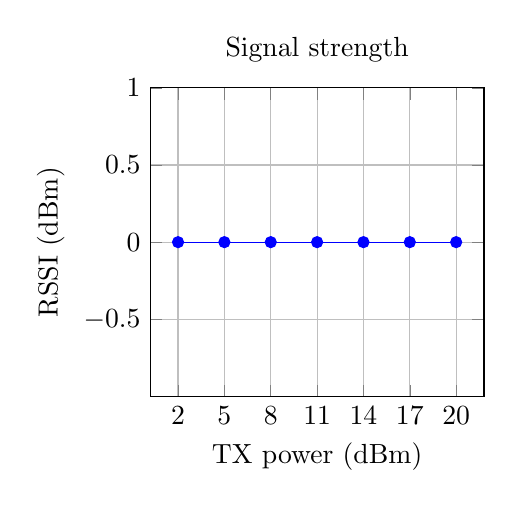
\begin{tikzpicture}
        \begin{axis}[
            width=0.48\textwidth, height=5.5cm,
            xlabel={TX power (dBm)}, ylabel={RSSI (dBm)},
            xtick={2,5,8,11,14,17,20}, grid=major,
            title={Signal strength}
        ]
            \addplot[mark=*, blue] coordinates {
                (2,0) (5,0) (8,0) (11,0) (14,0) (17,0) (20,0)
            };
        \end{axis}
    \end{tikzpicture}
    \hfill
    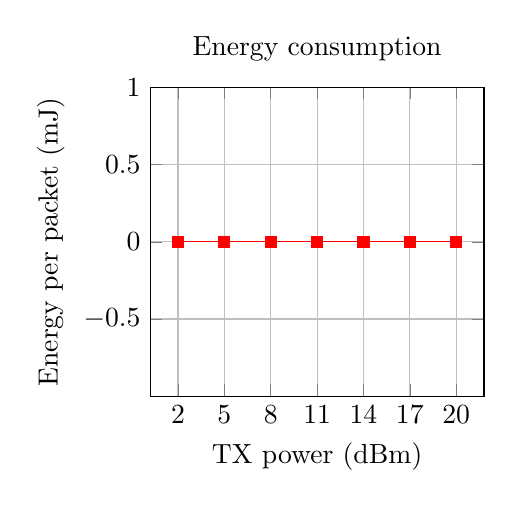
\begin{tikzpicture}
        \begin{axis}[
            width=0.48\textwidth, height=5.5cm,
            xlabel={TX power (dBm)}, ylabel={Energy per packet (mJ)},
            xtick={2,5,8,11,14,17,20}, grid=major,
            title={Energy consumption}
        ]
            \addplot[mark=square*, red] coordinates {
                (2,0) (5,0) (8,0) (11,0) (14,0) (17,0) (20,0)
            };
        \end{axis}
    \end{tikzpicture}
    \caption{RSSI at the receiver (left) and energy per packet at the
             transmitter (right) as a function of the transmission power.}
    \label{fig:txpower-results}
\end{figure}

\subsubsection{Discussion}

\paragraph{Time on air.} \todo{Check that $t_{\text{air}}$ is constant for all the power levels and compare it with the expected 41~ms. Explain any difference (SPI overhead, \texttt{millis()} resolution).}

\paragraph{Signal strength.} \todo{Comment on how the RSSI changes with the power. Is the relation linear (about 1~dB per dB)? Does it saturate at high power because the boards are close? Were any packets lost at low power?}

\paragraph{Energy consumption.} \todo{Comment on how the current and the energy per packet grow with the power. Which levels are most expensive? How much more energy does 20~dBm need compared with 14~dBm?}

\paragraph{Trade-off.} \todo{Conclude which power level is the best choice for this deployment: the lowest one that still gives a reliable link with some margin. Remember that in the EU868 band the legal limit is usually 14~dBm ERP, so 17 and 20~dBm were only used for this lab test.}

\subsection{Bandwidth and data rate}
% ASSIGNED: JAUME / AARON
\tcmp{Variación de bandwidth / spreading factor; resultados en tabla o gráfica.}

\subsection{Quality of Service: packet loss vs.\ distance}
% ASSIGNED: JAUME / AARON
\tcmp{Medida de pérdida de paquetes a distintas distancias; resultados.}

\subsection{Discussion of the results}
\tcmp{Análisis conjunto de los resultados.}

% =====================================================================
\section{Answers to Guiding Questions}
\label{sec:questions}
% ASSIGNED: MARCOS / MIKA
% =====================================================================

%\begin{enumerate}[label=\textbf{Q\arabic*.}, leftmargin=*]
%    \item \textbf{How does LoRa compare to Wi-Fi and Bluetooth in terms of range and power consumption?}
%
%    \textbf{MARCOS:} LoRa trades speed for range and efficiency. Working in the sub-GHz band (868~MHz here) with chirp spread spectrum, it can reach several kilometres with very low power consumption, but it only offers a few kbps (about 11~kbps with our SF7/250~kHz configuration). Wi-Fi offers Mbps but only reaches tens of metres, needs an access point and is power-hungry (an ESP32 draws well over 100~mA while transmitting over Wi-Fi), while Bluetooth/BLE has low consumption but a range of only about 10--100~m. This is why the TX node can send small readings every few seconds without any network infrastructure.
%
%    \textbf{MIKA:} \tcmp{Respuesta}
%
%    \item \textbf{What are the trade-offs of using lower data rates in LoRa transmission?}
%
%    \textbf{MARCOS:} A lower data rate (higher spreading factor or narrower bandwidth) increases the receiver sensitivity, so the link reaches further and tolerates more noise. The price is a longer time on air, which roughly doubles with each step of the spreading factor (about 44~ms for our messages with SF7/250~kHz versus around 2~s with SF12/125~kHz). This means more energy per packet, a higher chance of collisions and fewer messages allowed under the 1\% duty cycle of the EU868 band, together with lower throughput and higher latency.
%
%    \textbf{MIKA:} \tcmp{Respuesta}
%
%    \item \textbf{How does increasing transmission power affect battery life and interference?}
%
%    \textbf{MARCOS:} A higher transmission power makes the power amplifier draw more current (for the SX1276, roughly 30~mA at 13~dBm versus about 120~mA at 20~dBm), so each packet costs more energy and the battery lasts less, while the gain in range is small (about +6~dB is needed to double the free-space distance). It also increases the interference with other devices sharing the ISM band and, if the boards are very close, it can saturate the receiver. The best practice is to use the lowest power that gives a reliable link, as encouraged by the EU868 limit of about 14~dBm ERP (see Section~\ref{sec:exp-txpower}).
%
%    \textbf{MIKA:} \tcmp{Respuesta}
%\end{enumerate}
%

\begin{enumerate}[label=\textbf{Q\arabic*.}, leftmargin=*]
    \item \textbf{How does LoRa compare to Wi-Fi and Bluetooth in terms of range and power consumption?}
 
    \textbf{MARCOS:} LoRa trades speed for range and low consumption. It can reach several kilometres while using very little energy, but it can only send small amounts of data slowly. Wi-Fi is much faster, but its range is limited to a building or a house, it needs an access point and it consumes much more energy. Bluetooth also consumes little, but its range is only a few tens of metres. This is why LoRa fits our case: the TX node only sends a small reading every few seconds and does not need any network infrastructure.
 
    \textbf{MIKA:} LoRa provides a significantly greater communication range than Wi-Fi
and Bluetooth in many practical IoT deployments, often reaching
hundreds of metres or several kilometres under suitable conditions.
Wi-Fi and Bluetooth are generally intended for shorter distances,
although their actual range depends on the hardware and environment.

LoRa is particularly suitable for transmitting small amounts of
sensor data over long distances while allowing devices to operate
with low average power consumption. Wi-Fi supports much higher data
rates but can consume more energy, while Bluetooth generally offers
lower power consumption for short-range communication, although this
depends on the Bluetooth version and operating mode.

For our ESP32 project, LoRa is appropriate because the boards only
need to exchange small sensor measurements periodically, rather than
transmit large amounts of data. This allows long-range communication
without requiring the high data rates provided by Wi-Fi.

 
    \item \textbf{What are the trade-offs of using lower data rates in LoRa transmission?}
 
    \textbf{MARCOS:} Sending the data more slowly makes the signal easier for the receiver to detect, so the link reaches further and resists noise better. The price is that each message takes longer to send. The radio stays on for more time, so every message costs more energy, there is a higher chance of colliding with other transmissions, and the legal limits on how long a device may transmit allow fewer messages per hour. The data also arrives with more delay.
 
    \textbf{MIKA:} Reducing the LoRa data rate generally increases receiver sensitivity and potential communication range, but also increases packet transmission time. This is commonly achieved by increasing the spreading factor or reducing the bandwidth.

Longer transmission times increase the energy required to send each message and occupy the shared radio channel for longer, increasing the possibility of packet collisions. Therefore, a lower data rate does not necessarily result in lower energy consumption per message.

In our configuration, SF7 and a bandwidth of 250~kHz favour shorter transmission times. This is appropriate for small sensor messages, provided that the receiver can decode them reliably. A higher spreading factor could be used if greater range or better sensitivity were required.
 
    \item \textbf{How does increasing transmission power affect battery life and interference?}
 
    \textbf{MARCOS:} A higher transmission power gives a stronger signal, but the radio needs more current to send it, so each message costs more energy and the battery lasts less. In exchange, the extra range is small. A stronger signal also interferes more with other devices using the same frequency band and, if the boards are very close, it can even overload the receiver. For this reason, the best practice is to use the lowest power that still gives a reliable link, which is what the power experiment of Section~\ref{sec:exp-txpower} tries to find.
 
    \textbf{MIKA:} Increasing transmission power can improve the received signal strength and extend the potential communication range. However, it also generally increases the energy drawn by the radio during transmission, potentially reducing battery life.

For example, increasing output power from 10~dBm to 17~dBm increases the transmitted radio-frequency power from 10~mW to approximately 50~mW. The battery consumption does not necessarily increase by the same factor, since the radio's efficiency and other power requirements must also be considered.

Higher transmission power can also increase interference for other devices sharing the same or overlapping frequencies. Therefore, the appropriate strategy is to use the minimum power that maintains a reliable connection between the two ESP32 boards.

In our project, RSSI measurements and packet reception tests can help determine whether the selected power provides sufficient reliability without unnecessary energy consumption or interference. The final setting must also comply with the applicable radio regulations.
\end{enumerate}

% =====================================================================
\section{Conclusions}
\label{sec:conclusions}
% ASSIGNED: TODOS
% =====================================================================
\tcmp{Conclusiones conjuntas.}

\end{document}